%%%%%%%%%%%%%%%%%%%%%%%%%%%%%%%%%%%%%%%%%%%%%%%%%%%%%%%%%%%%%%%%%%%%%%%%%%%%%%%%%%%%%%%%%%%%%
%%									Chapitre 1											%
%%%%%%%%%%%%%%%%%%%%%%%%%%%%%%%%%%%%%%%%%%%%%%%%%%%%%%%%%%%%%%%%%%%%%%%%%%%%%%%%%%%%%%%%%%%%%
\chapter{Exploration de l'entreprise}
	\minitoc

%%%%%%%%%%%%%%%%%%%%%%%%%%%%%%%%%%%%%%%%%%%%%%%%%%%%%%%%%%%%%%%%%%%%%%%%%%%%%%%%%%%%%%%%%%%%%




% Début du chapitre

\section{Le rôle du laboratoire Soleil}

	\subsection{Secteur d'activité}
				Le laboratoire SOLEIL est une entreprise du secteur tertiaire. Il est installé sur le plateau de Saclay en région parisienne. L'objectif du laboratoire est la recherche fondamentale.
				
				Des personnes venant du monde entier viennent faire des recherches au synchrotron SOLEIL parce qu'il y a peu d'équipement aussi performants pour l'étude de la matière dans le monde. Il y en a deux en France. Le second, qui se trouve à Grenoble, est lui un synchrotron européen donc une partie appartient aux français et le reste à d'autre pays européen.

	\subsection{Moyens}
		
		\subsubsection{Personnels}
				En décembre 2015, 432 personnes travaillent au laboratoire SOLEIL. L'âge moyen des salariés est de 44 ans. 5 personnes souffrant d'un handicap travaillent à SOLEIL. L'ancienneté moyenne des salariés est de 8 ans.
				
				75\% , c'est à dire 267, des salariés SOLEIL sont des hommes~: 150 sont cadres et 117 sont non cadres.
				
				25\% , donc 80 des personnes embauchées à SOLEIL sont des femmes~: 42 sont cadres et 38 sont non cadres.


		\subsubsection{Équipements}
			
			\paragraph{L'accélérateur d'électrons}
				La plus grande machine du synchrotron SOLEIL est l'accélérateur d'électrons. La lumière émise par les électrons tournant dans l'accélérateur permet d'observer la matière. 
				
				Les électrons sont produits puis accélérés de la façon suivante : 
				\begin{itemize}
					\item Un canon, nommé le LINAC, envoie une grande énergie électrique qui va séparer les électrons des atomes. Les électrons sortent du canon à une vitesse de 100 Méga-électrons-Volt.  
					\item Dans le booster, ils atteignent une énergie de 2750 Méga-électrons-Volt. Quand les électrons ont atteint cette vitesse, ils sont envoyés dans l'anneau de stockage qui est un tube fermé de cinq centimètres de diamètre où ils tournent pendant plusieurs heures à une vitesse très proche de celle de la lumière. 

					\item L'anneau de stockage est constitué d'une succession de parties droites et de virages où les électrons tournent et subissent des accélérations. 
				\end{itemize}


				Quand les électrons tournent, ils libèrent des photons, c'est à dire de la lumière. Ce processus est utilisé par 7 lignes de lumière. Pour les autres lignes de lumière, ce sont des onduleurs qui accélèrent les électrons pour qu'ils émettent des photons. Ces photons vont être utilisés par les scientifiques qui vont expérimenter la réaction de la lumière sur des objets ou inversement. 
				\begin{figure}[h]
 				 \centering
 				 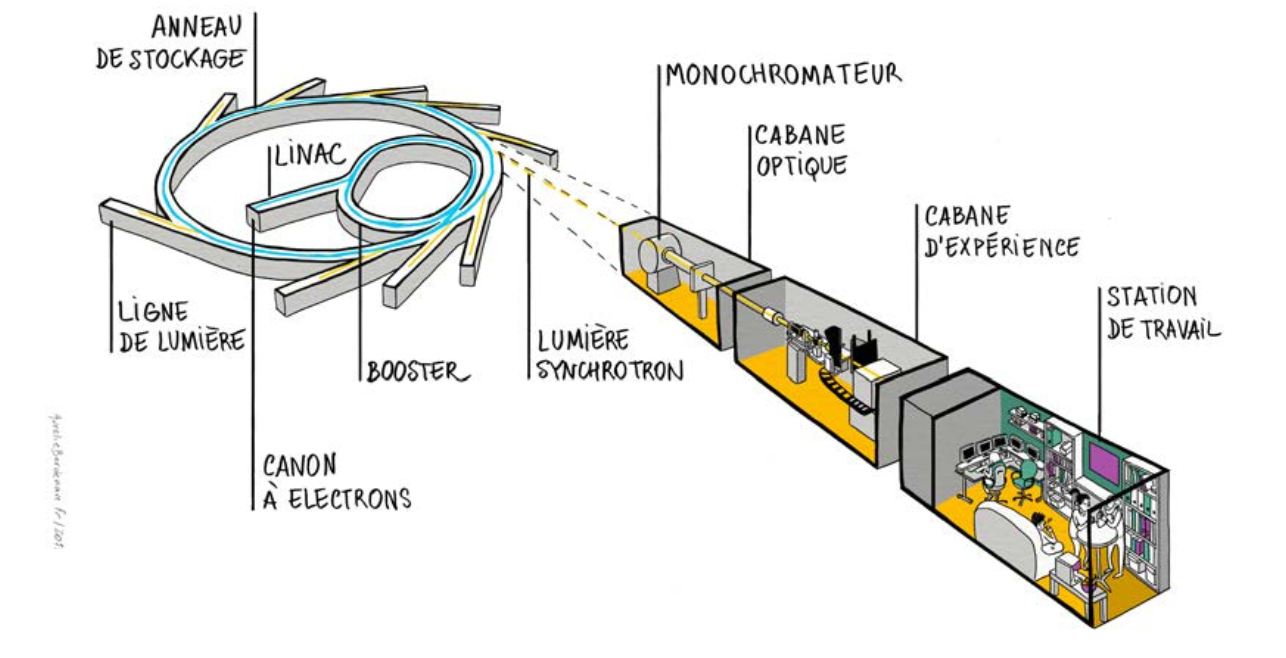
\includegraphics[width=16cm]{Chapitre1/ImageLigne.png}
 				 \caption{Une ligne de lumière}
 				 \label{Ligne-Lumiere}
				\end{figure}				
				\par Chaque ligne est composée de trois cabanes~(cf. figure~\ref{Ligne-Lumiere})~: la cabane optique, la cabane d'expériences et la cabane de vie. 
				Dans la cabane optique, on trouve des miroirs déviant la lumière. La cabane d'expériences est l'endroit où on pose l'échantillon à observer et la cabane de vie est l'endroit où on observe l'échantillon et où les scientifiques règlent la caméra. 
				
				\par Les photons sont émis avec des énergies différentes. Plus ils ont d'énergie et plus la lumière a une longueur d'onde courte et permet d'étudier la lumière à petite échelle (\ref{Longueur-Onde}). La plus petite longueur d'onde produite par le synchrotron SOLEIL est de l'ordre du nanomètre (Rayons X).

				\begin{figure}[h]
 				 \centering
 				 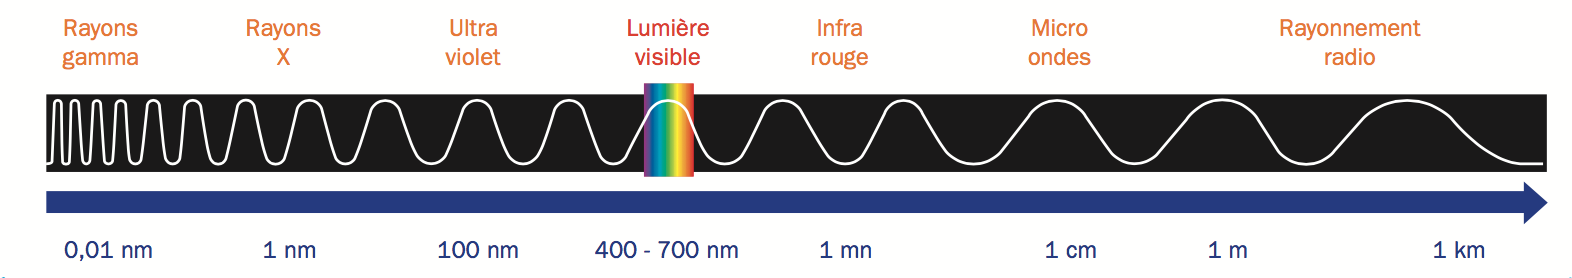
\includegraphics[width=16cm]{Chapitre1/LongueursOnde.png}
 				 \caption{Les longueurs d'onde de la lumière}
 				 \label{Longueur-Onde}
				\end{figure}				

			\paragraph{Les Aimants}
				\begin{figure}[h]
 				 \centering
 				 \reflectbox{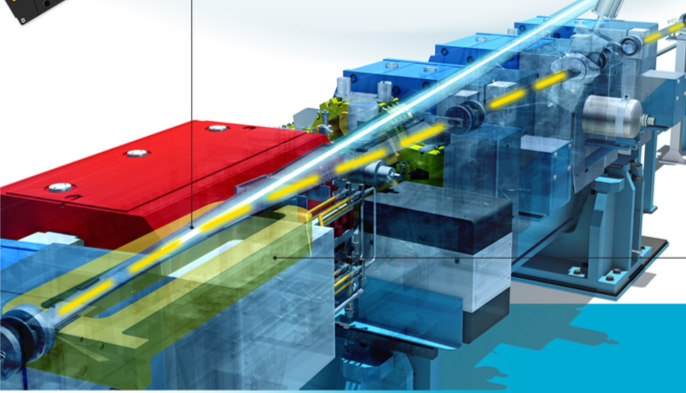
\includegraphics[width=16cm]{Chapitre1/Lesaimants}}
 				 \caption{Les aimants de l'anneau de stockage}
				\end{figure}

				Pour guider les électrons sur une trajectoire circulaire, des aimants sont utilisés. Plusieurs sortes d'aimants sont utilisés à SOLEIL.\par Il y a le dipôle, qui comporte deux aimants et qui dévie les électrons du côté choisi. 
				\par Les quadripôles servent à resserrer les électrons entre eux parce que dans les virages, ils ont plus de place et ont tendance à s'éloigner les uns des autres. En effet, deux charges négatives se repoussent. Les aimants nommés sextupôles font la même chose que les quadripôles mais plus précisement. 
				\par Pour alimenter les aimants en électricité, on utilise des alimentations qui sont contenus dans de très grande armoires. Il existe 32 dipôles, 160 quadripôles et 120 sextupôles au synchrotron SOLEIL. 
				\par Dans le booster, on utilise des dipôles et des quadripôles. Dans l'anneau de stockage, on utilise des sextupôles, des dipôles et des quadripôles plus puissants. 

			\paragraph{Autres équipements}
				Le synchrotron SOLEIL possède trois imprimantes 3D avec lesquelles sont fabriquées de petites pièces.

				Dans chaque salle, on voit un ou plusieurs ordinateurs. Dans la salle de commande, les cabanes de vie, les bureaux d'ingénieurs, des dessinateurs projecteurs, des mécaniciens, des scientifiques... 

				Les aligneurs disposent d'appareils spécifiques pour positionner précisement tous les équipements des lignes de lumières~:
				\begin{itemize}	
				 \item des niveaux (comme ceux utilisés en travaux publics) pour prendre des mesures~;
				 \item des théodolites qui servent à mesurer des angles.
				\end{itemize}

				Des pompes sont utilisées par les videurs pour faire le vide dans les tubes de l'accélérateur d'électrons.




%\section{Deuxième paragraphe}
%\blindtext

%\bibliographystyle{francaissc}
%\bibliography{Chapitre1/Biblio}